%%%%%%%%%%%%%%%%%%%%%%%%%%%%%%%%%%%%%%%%%%%%%%%%%%%%%%%%%%%%%%%%%%%%%%%%%%%%%%%%
%Objetivo: Descrever os principais conceitos relativos a Manutenção de Software
%		   envolvidos na dissertação
%Autores: Vagner Clementino <vagnercs@dcc.ufmg.br>
%		  Rodolfo Resende <rodolfo@dcc.ufmg.br>
%Criação: Ter Set 13 19:22:37 BRT 2016
%Modificação: Dom Set 25 15:53:04 BRT 2016
%Revisão:  Ter Set 20 19:13:49 BRT 2016
%%%%%%%%%%%%%%%%%%%%%%%%%%%%%%%%%%%%%%%%%%%%%%%%%%%%%%%%%%%%%%%%%%%%%%%%%%%%%%%%

\chapter{Manutenção de Software: Uma Visão Geral}
\label{ch:visao-geral-manutencao}

Uma tendência natural do software é evoluir a fim de atender aos novos
requisitos e alterações do ambiente no qual ele está inserido. Em uma série de
estudos, Lehman propõe um conjunto de leis sobre a evolução do software. Dentre
elas podemos destacar as leis da Mudança Contínua (Continuing Change) e da
Complexidade Crescente (Increasing complexity). A primeira diz que um programa
que é utilizado em um ambiente real deve mudar ou se tornará progressivamente
menos útil~\cite{lehman1980understanding}. A lei da Complexidade Crescente
(Increasing complexity) afirma que quando um sistema em evolução muda, sua
estrutura tende a se tornar mais complexa. Nesta situação, recursos extras devem
ser disponibilizados a fim de preservar e simplificar a estrutura do
software~\cite{lehman1980understanding}. As leis de Lehman tem sido validadas,
especialmente aquelas relacionadas a tamanho e complexidade do software. Em um
trabalho sobre o tema Yu \& Mishra~\cite{{yu2013empirical}} examinaram de forma
empírica as Leis de Lehman em relação a evolução da qualidade do software. O
estudo demonstrou que com base na métrica proposta que a qualidade de um produto
de software declinará ao menos que uma restruturação é realizada.

Conforme exposto, a mudança em um produto de software é inevitável. Desta forma,
é importante a existência de uma área de estudo preocupada com o gerenciamento e
controle destas mudanças. Dentro do escopo da Engenharia de Software esta tarefa
fica a cargo da Manutenção de Software.  Nas próximas seções discutimos os
conceitos básicos que mostram onde e como a Manutenção se encaixa dentro da
Engenharia de Software. São apresentados os conceitos que fazem da Manutenção de
Software uma disciplina distinta.

%Percebida a importância do processo de manutenção de software, alguns trabalhos
%foram propostos visando mensurar o seu custo bem como propor processos com o
%objetivo de reduzir o esforço envolvido neste tipo de atividade.
%
%No trabalho de Herrin~\cite{Herrin:1985:SMC:323287.323383} foi proposto um
%modelo matemático com o objetivo de avaliar o impacto financeiro no orçamento
%de uma universidade devido às atividades de manutenção no sistema de
%processamento de dados da instituição. O modelo propõe que o valor disponível
%para desenvolvimento de um novo sistema é função inversa do custo de manutenção
%do software existente. Desta forma, o fato de se manter um sistema durante
%muito tempo poderá impossibilitar a aquisição ou mesmo o desenvolvimento de um
%novo.
%
%No estudo de Hirota et al.~\cite{hirota1994approach} é proposta a utilização da
%técnica Análise de Ripple para estimar o custo da manutenção de software. O
%termo ``efeito Ripple'' foi utilizado pela primeira vez em um artigo publicado
%por Haney~\cite{haney1972module} para descrever a forma que a mudança em um
%módulo poderia causar alterações em outras partes do
%sistema~\cite{bilal2005using}. A Análise Ripple é, portanto, uma técnica para
%analisar o fluxo de dados de variáveis dentro de um determinado programa. Os
%valores retornados pela aplicação do método são denominados Complexidade de
%Ripple. Os resultados demostraram que a Complexidade de Ripple está mais
%relacionada ao entendimento do software do que as métricas padrão, como linhas
%de código, complexidade ciclomática e pontos de função. Desta forma, a
%Complexidade de Ripple poderia ser utilizada, por exemplo, para predizer os
%custo de manutenção de um sistema, bem como a necessidade de substituição do
%mesmo.
%
%Mediante o uso de Redes Neurais Shula \& Misra
%\cite{Shukla:2008:ESM:1342211.1342232} propõe um estudo para medir o custo de
%manutenção de software. O trabalho discute a utilização de outras métricas além
%de linha de código e pontos de função para medir  tamanho e custo do processo
%de manutenção. Os resultados demonstraram a possibilidade de construir um
%modelo para medir o custo utilizando Redes Neurais. Contudo, os resultados são
%sensíveis a escolha da arquitetura e parâmetros de treino, os quais idealmente
%deveriam ser preparados por um especialista no sistema (oráculo).
%
%A dinamicidade do ambiente de negócios tem levado a diversas organizações a
%adotar as metodologias propostas pelos agilistas pelo fato delas auxiliarem no
%atendimento das exigências do cliente~\cite{Devulapally2015}. Esta tendência é
%mais forte no desenvolvimento de software e nos últimos anos vem ocorrendo de
%forma gradativa na manutenção.
%
%No trabalho de Kajko-Mattsson \& Nyfjord~\cite{4755767} foi proposto um modelo
%ágil para manutenção que apropria diferentes práticas do Extreme Programming e
%do Scrum. Segundo os autores a junção desta duas metodologias possibilita a
%inclusão de práticas úteis tanto do ponto de vista do gerente do projeto bem
%como dos desenvolvedores. O modelo encoraja diversas práticas tais como
%\textit{product backlog}, testes antes da codificação, planejamento iterativo,
%dentre outras.
%
%A adoção na manutenção de software de algumas práticas propostas pelos
%agilistas foram analisadas durante 08 meses em estudo realizado por Svensson \&
%Host~\cite{1402140}. Ao utilizar o Extreme Programming (XP) no processo de
%manutenção os autores concluíram que é muito difícil fazer uso do XP sem que
%sejam realizadas adequações no desenho de diversas práticas para desta forma
%adequar às necessidades do time de desenvolvimento.
%
%O estudo Heeager \& Rose~\cite{Heeager2015} propõe um conjunto de nove
%heurísticas com o objetivo de ajudar aos profissionais da manutenção de
%software na adoção de práticas propostas pelos agilistas. O trabalho consistiu
%da inclusão do Scrum na rotina de trabalho do departamento de manutenção de
%software de uma organização de grande porte. Os autores argumentam que os
%métodos ágeis, quando aplicado ao trabalho de desenvolvimento, têm certas
%características relativamente bem compreendidas, no entanto o trabalho de
%manutenção difere do de desenvolvimento em certos aspectos e, portanto, é
%desafiador a implementação de métodos ágeis em um departamento de manutenção.
%
\section{Conceitos Fundamentais}
\label{sec:conceitos_basicos}

Esta seção introduz os conceitos e terminologias que ajudam no entendimento do
papel e escopo da Manutenção de Software. De uma maneira geral, podemos definir
atividade de manter software como a totalidade das ações necessárias para
fornecer suporte a um produto de software. Entretanto, encontramos na literatura
outras definições mais elaboradas sobre a área.

Manutenção de Software é definida pela IEEE 1219~\cite{ISO-1219-1998}-~Padrão para a
Manutenção de Software, como a modificação de um produto de software após a sua
entrega com o objetivo de corrigir falhas, melhorar o desempenho ou outros
atributos com a finalidade de adaptar o software as modificações ambientais. O
padrão cita a ocorrência de atividade de manutenção antes da entrega
propriamente dita, contudo, de forma bastante superficial.

Posteriormente a IEEE/EIA 12207~-~Padrão para o Processo de Ciclo de Vida do
Software~\cite{{ISO/IEC-12207-2008}} retrata a manutenção como um dos principais processos no
ciclo de vida do software. Em seu texto a manutenção é vista como atividade de
modificação do código e da documentação associada e ocorre devido a algum
problema ou necessidade de melhoria~\cite{IEEEComputerSociety:2014:GSE:2616205}.
Por outro lado a ISO/IEC 14764~-~Padrão para Manutenção de
Software~\cite{1703974}enfatiza aspectos pré-entrega da manutenção, como por
exemplo o planejamento.

De maneira relacionada, \textit{Manutenibilidade} é a propriedade de um sistema
ou componente de software em relação ao grau de \textit{facilidade} que ele pode
ser corrigido, melhorado ou adaptado~\cite{{159342}}. A
ISO/IEC~9126~-~01~\cite{ISOIEC9126} define a Manutenibilidade como uma
característica de qualidade do processo de Manutenção.

Apesar das diversas definições para Manutenção de Software é possível
identificar dois aspectos comuns: manter e evoluir. O conceito de evolução de
software carece de uma definição padrão na literatura, contudo, pesquisadores e
profissionais utilizam o termo como substituto preferido para
manutenção~\cite{Bennett:2000:SME:336512.336534}. Embora exista o entendimento
que os processos de manutenção e evolução possuem características distintas, não
está no escopo desta dissertação discutir e apresentar tais diferenças. Neste
sentido, utilizamos os termos \textit{manter} e \textit{evoluir} software de
forma intercambiáveis. Caso em algum contexto haja a necessidade de
diferenciação, ela será discutida.

A Manutenção é necessária para garantir que o software seja capaz de satisfazer
os requisitos dos usuários. Neste sentido, a atividade de manter software pode
ser vista como um desenvolvimento contínuo, sobretudo, pelo fato que alguns
sistemas nunca estão completos e continuam a evoluir.

\section{Requisição de Mudança}
\label{sec:requisição_de_mudanca}

As manutenções em software podem ser divididas em \textit{Corretiva, Adaptativa,
	Perfectiva e Preventiva}~\cite{Lientz:1980:SMM:601062,159342}.  A Manutenção
Corretiva lida com a reparação de falhas encontradas. A Adaptativa tem o foco na
adequação do software devido à mudanças ocorridas no ambiente em que ele está
inserido. A Perfectiva trabalha para detectar e corrigir falhas latentes. A
Preventiva preocupa com atividades que possibilitem aumento da manutenibilidade
do sistema.  A \textit{ISO 14764}~\cite{1703974} propõe a divisão da tarefa de
manutenção nos quatro tipos descritos anteriormente e propõe que exista um
elemento comum denominado Requisição de Mudança que representa as
características comuns a todas aqueles tipos de manutenção.o A
Figura~\ref{fig:modification-request} exibe a classificação das RM's conforme
discutido pela ISO\@.

\begin{figure}[hbtp] \centering 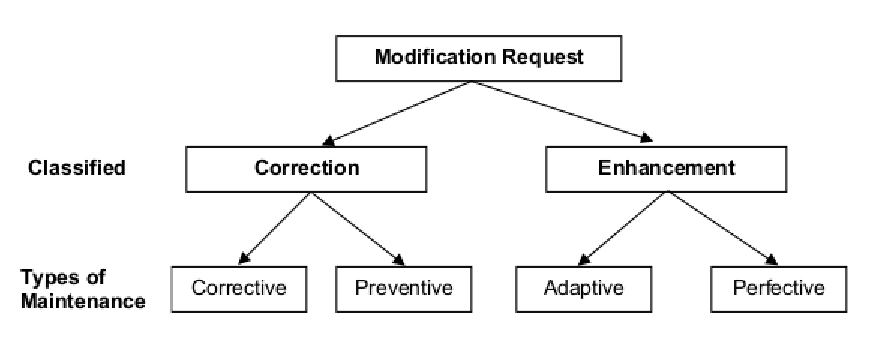
\includegraphics[width=.75\textwidth]
	{chapter-intro/img/modification_request.eps} \caption{Tipos de manutenção
		segundo a norma ISO/IEC 14764. Extraído de~\cite{1703974}}
	\label{fig:modification-request} \end{figure}

A ISO/IEC 14764 classifica as manutenções adaptativas e perfectivas como
melhorias e agrupa as manutenções corretivas e preventivas em uma única
categoria de correção, conforme exibido na
Tabela~\ref{tab:categorias_requisicao_mudanca}. A manutenção preventiva é mais
frequentemente realizada em produtos de software onde atributos de segurança são
mais críticos.
%At Modification requests are logged and tracked, the impact of proposed changes
%is determined, code and other software artifacts are modified, testing is
%conducted, and a new version of the software product is released

\begin{table}[htpb] \centering 	\begin{tabular}{l|l|l|} \cline{2-3} &
		\textbf{Correção} & \textbf{Melhoria} \\ \hline
		\multicolumn{1}{|l|}{\textbf{Pró-ativa}} & Preventiva & Perfectiva \\
		\hline \multicolumn{1}{|l|}{\textbf{Reativa}} & Corretiva & Adaptativa
		\\ \hline \end{tabular}\caption{Categorias da Requisição de Mudanças.
		Adaptado de
		SWEBOK~\cite{4425813}}\label{tab:categorias_requisicao_mudanca}
\end{table}

Em síntese, apesar das diferentes nomenclaturas existentes na literatura
(demanda, bug, defeito, bilhete, tíquete, requisição de modificação, relato de
problema) uma Requisição de Mudança representa o relato, independente de sua
estrutura, que têm por objetivo gerar a manutenção ou evolução do software.

\section{O processo de Manutenção de Software}
 \label{sec:o_processo_de_manutecao_de_software}

Um Processo de Software é o conjunto de atividades, métodos, práticas e
transformações utilizadas para desenvolvê-lo ou mantê-lo bem como seus artefatos
associados~\cite{paulk1993key}. Independente do contexto em que a manutenção
ocorra é importante que o processo esteja bem definido. Existe na literatura a
proposição de alguns modelos do processo de manutenção de software,
especialmente baseado em uma visão tradicional no qual desenvolvimento e
manutenção possuem uma clara separação. Recentemente os métodos propostos pelos
agilistas vêm sendo utilizados para manter software. Esta tendência surge da
demanda crescente por serviços de manutenção com um retorno mais rápido para o
usuário.

Nas próximas seções apresentamos alguns modelos encontrados na literatura na
perspectiva tradicional, ao mesmo tempo descrevemos propostas do uso da
metodologia dos agilistas na manutenção de software.

\subsection{Manutenção de Software Tradicional}
\label{subsec:manutenção_de_software_tradicional}

Em resumo, um processo de manutenção de software descreve as atividades e suas
respectivas entradas e saídas. Alguns modelos são descritos nos padrões IEEE
1219 e ISO/IEC 14764. O processo especificado no Padrão para Manutenção de
Software (IEEE-~1219) indica que as atividade de manutenção de software iniciem
após a entrega do produto de software. O padrão também discute itens para fins
de planejamento da manutenção. As atividades que compõe o processo são
apresentas na Figura~\ref{fig:ieee-1219-processo-man-software}.

\begin{figure}[htpb] \centering
	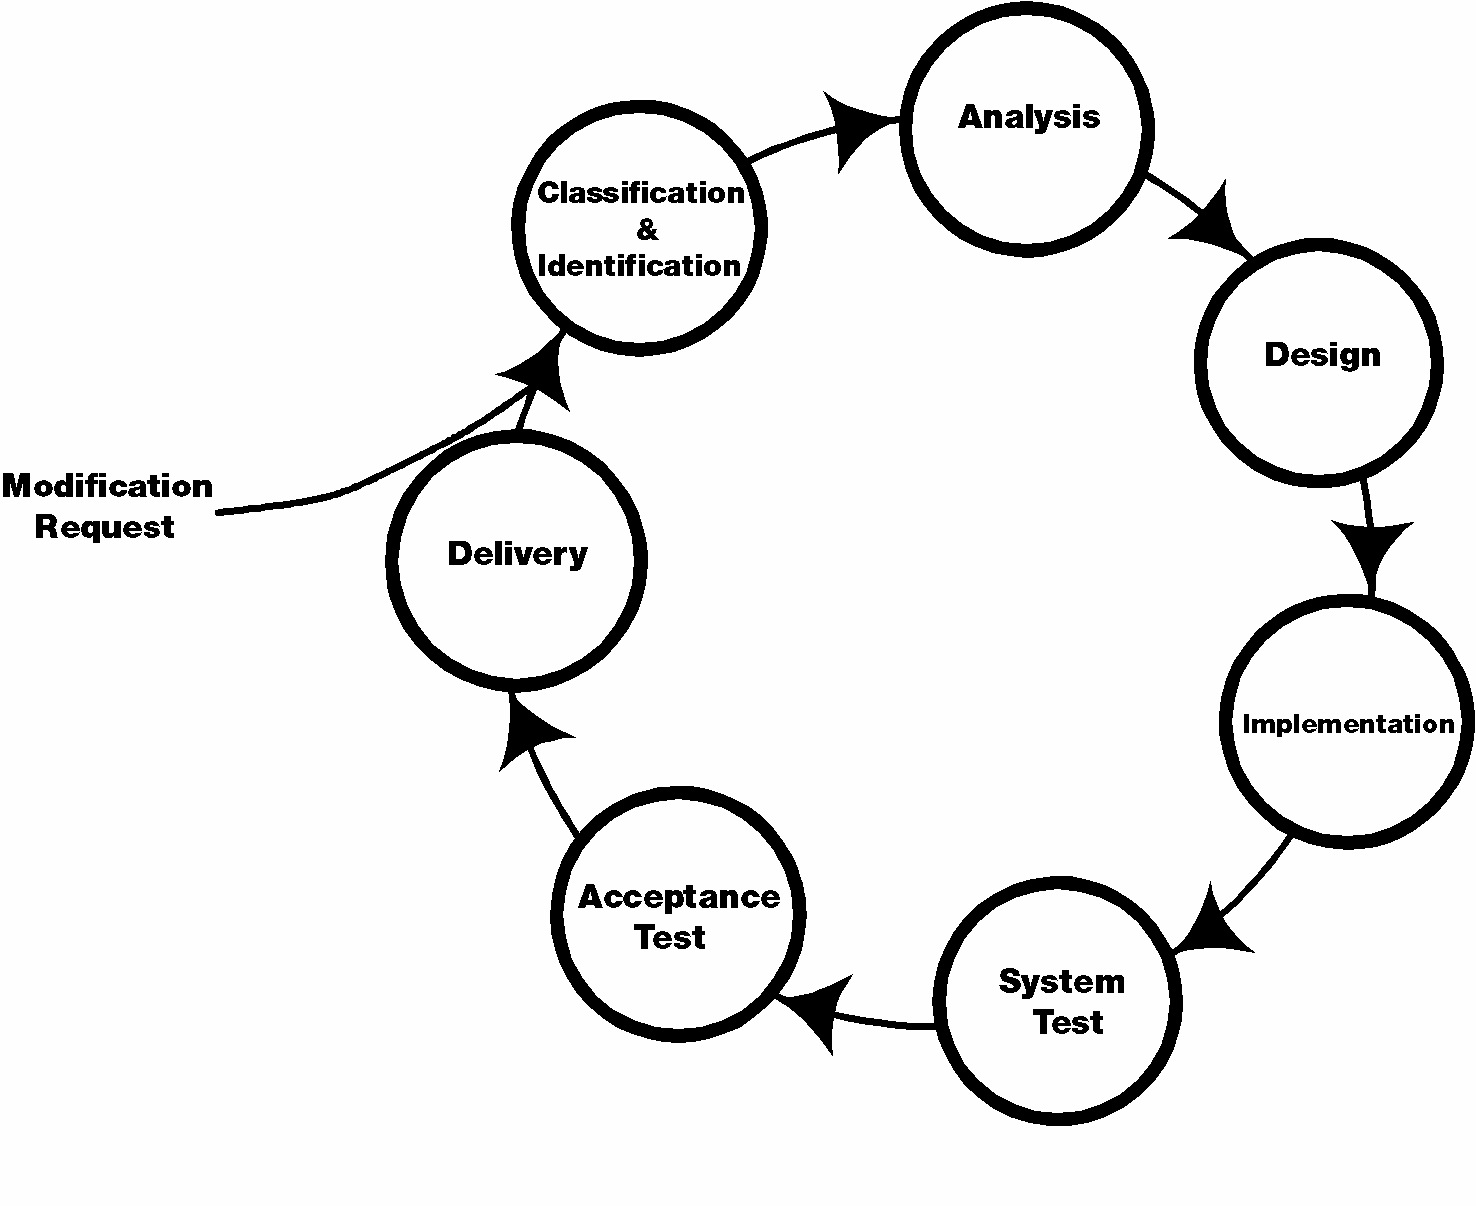
\includegraphics[width=0.7\linewidth]
	{chapter-manutencao-software-visao-geral/img/ieee-1219-98-processo-manutencao.png}
	\caption{IEEE 1219 -~Processo de Manutenção de Software}
	\label{fig:ieee-1219-processo-man-software} \end{figure}

De maneira relacionada, na ISO/IEC 14764 as atividades que compõe o processo são
similares aquelas propostas na IEEE-~1219, exceto pelo fato que elas são
agregadas de uma forma diferente. O processo descrito na ISO/IEC~14764 são
exibidas na Figura~\ref{fig:ieee-14764-processo-manutencao}

\begin{figure}[htpb] \centering
	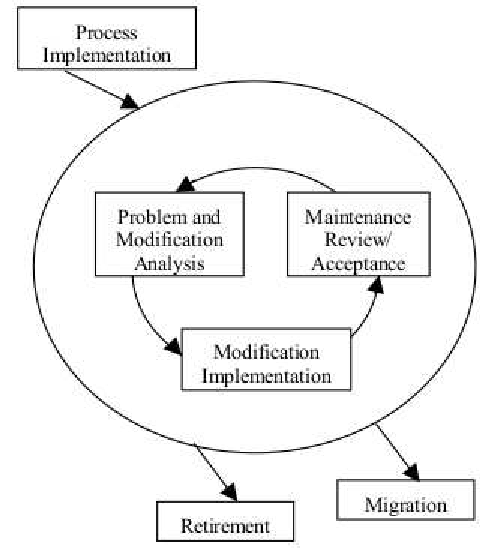
\includegraphics[width=0.7\linewidth]
{chapter-manutencao-software-visao-geral/img/ieee-14764-processo-manutencao.pdf}
	\caption{ISO/IEC~14764 Processo de Manutenção de Software}
	\label{fig:ieee-14764-processo-manutencao} \end{figure}

As atividades de manutenção propostas na ISO/IEC 14764 são detalhadas em tarefas
conforme apresentadas a seguir:

\begin{itemize} \item Implementação do Processo \item Análise e Modificação do
		Problema \item Aceitação e Revisão da Manutenção \item Migração \item
		Aposentadoria do Software	\end{itemize}

É possível notar que algumas atividades realizadas durante a manutenção de
software são similares a a outras presentes no desenvolvimento de software, como
por exemplo, análise de desempenho, codificação, teste e documentação. Outra
atividade comum à manter e desenvolver software é o gerenciamento dos
requisitos. Nas duas situações os profissionais responsáveis por controlar os
requisitos devem atualizar documentação  por conta de alterações ocorridas no
código fonte. Por outro lado certas atividades estão vinculadas apenas ao
contexto da manutenção de software. Dentre elas podemos destacar:

\begin{description}
	\item[Suporte ao Usuário] Função de ajuda ao usuário final
		que podem disparar ações tais como avaliação e priorização das
		Requisições de Mudanças
   	\item [Análise de Impacto] \todo{Descreve melhor
			análise de impacto}
   	\item [Suporte ao Uso de Software] Ajuda aos
		usuários final com relação a determinada requisição de informação
		(regras de negócio, validação e requisição de relatório)
	\item [Acordo de Nível de Serviço] Definição de um nível mínimo de qualidade que a
		atividade de manutenção deve ser realizada.
\end{description}

\subsection{Manutenção de Software com Método dos Agilistas}
\label{sub:manutenção_de_software_com_método_dos_agilistas}

Grande parte da literatura de manutenção de software trata de técnicas e
metodologias tradicionais da Engenharia de Software. Entretanto, é possível
verificar um protagonismo das práticas propostas pelos agilistas em projetos de
sucesso, mesmo em áreas não relativas à Tecnologia da
Informação~\cite{Serrador2015}. Neste contexto, verifica-se uma tendência que os
departamentos dedicados à manutenção de software se mostrem interessados nas
metodologias dos agilistas e que tenham vontade de experimentá-las em suas
atividades \cite{Heeager2015}.

Apesar da maioria dos textos em Engenharia de Software tratarem desenvolvimento
e manutenção como atividades com natureza distintas, esta última pode adaptar
características da primeira visando a melhoria do seu desempenho. Dentre as
práticas propostas pelos agilistas passíveis de serem utilizadas em tarefas de
manutenção é possível citar o desenvolvimento iterativo, maior envolvimento do
cliente, comunicação face a face, testes frequentes, dentre outras.

Alguns resultados demonstram certa dificuldade para implantação da metodologia
dos agilista na manutenção de software~\cite{1402140}. Um dos possíveis
problemas é a necessidade de adequação das práticas da organização de modo que a
se adequar as necessidades do time de desenvolvimento.  Estudo apresentam
resultados relativos à melhorias no aprendizado e produtividade da equipe
mediante o aumento da moral, encorajamento e confiança entre os desenvolvedores,
o que propicia uma alta motivação durante o processo de manutenção de
software~\cite{Choudhari:2014:EIM:2557833.2557845}.

\section{Ferramentas de Gerenciamento de Requisições de Mudança (FGRM)}
\label{sec:ferramentas_de_gerenciameto_de_requisições_de_mudança}

Dentro da disciplina de Gerenciamento da Configuração do Software a atividade de
controle de configuração é responsável por gerenciar mudanças ocorridas durante
o ciclo de vida de um produto de software. Tais ações incluem determinar quais
alterações serão feitas, definir a autoridade responsável por autorizar certos
tipos de mudança e aprovar desvios relativos aos requisitos iniciais do
projeto~\cite{4425813}. De uma forma mais ou menos estruturada este tipo de
processo ocorre em diferente tipos de projeto de software, seja ele dentro de um
processo de manutenção tradicional ou mesmo naqueles que utilizam os métodos
propostos pelos agilistas.

Por conta do volume das Requisições de Mudança se faz necessária a utilização de
ferramentas com o objetivo de gerenciá-las. Esse controle é geralmente realizado
por Sistemas de Controle de Demandas (SCD)- Issue Tracking Systems, que auxiliam
os desenvolvedores na correção de forma individual ou colaborativa de defeitos
(bugs), no desenvolvimento de novas funcionalidades, dentre outras tarefas
relativas à manutenção de software. Não existe na literatura uma nomenclatura
comum para este tipo de ferramenta. Em alguns estudos é possível verificar nomes
tais como Sistema de Controle de Defeito - Bug Tracking Systems, Sistema de
Gerenciamento da Requisição - Request Management System, Sistemas de Controle de
Demandas (SCD)- Issue Tracking Systems e diversos nomes afins. Todavia, de modo
geral, o termo se refere as ferramentas utilizadas pelas organizações para
\textit{gerir as Requisições de Mudança}. Estas ferramentas podem ainda ser
utilizadas por gestores, analistas de qualidade e usuários finais para
atividades tais como gerenciamento de projetos, comunicação, discussão e
revisões de código. Neste trabalho utilizaremos o termo \texttt{Ferramentas de
	Gerenciamento de Requisições de Mudança} (FGRM) ao referimos a este tipo de
ferramenta.

No últimos anos alguns estudos discutem o fato que as FGRM's não apenas ajudam
as organizações gerenciar, atribuir, controlar, resolver e arquivar Requisições
de Mudança. Em alguns casos, este tipo de ferramenta se tornou o ponto focal
para comunicação e coordenação para diversas partes interessadas, dentro e além
da equipe de manutenção~\cite{Bertram:2010:CCB:1718918.1718972}.  As FGRM's
também servem como um repositório central para monitorar o progresso da RM,
solicitar informações adicionais da pessoa responsável por redigir a requisição
e o ponto de discussão para potenciais soluções um
bug~\cite{zimmermann2009improving}.

Em projetos de código aberto, as FGRM são uma importante parte de como o time
interage com comunidade de usuários. Como consequência é possível observar o
fenômeno da participação dos usuários no processo de solução da RM: eles não
apenas submetem a RM, mas também participam na discussão de como resolvê-la.
Desta forma, o usuário final ajuda tomar as decisões sobre a direção futura do
produto de software~\cite{breu2010information}.

Conforme exposto as FGRM desempenham um papel que vai além de gerenciar as
Requisições de Mudança.  Neste sentido, é importante estudar este tipo de
software em busca de como melhorá-las de modo a atender as diversas necessidades
dos seus usuários. Contudo, é importante avaliar as novas funcionalidades
propostas na literatura ou ainda mesmo a melhoria das já existentes. Uma
possível forma de melhoria é através do uso de extensões. Na próxima seção
discutiremos esta propriedade de algumas FGRM's que permitem a inclusão e
modificação de funcionalidades e comportamentos da ferramenta segundo as
necessidades do usuário.

\subsection{Extensões em FGRM} \label{subsec:extensoes_fgrm}

Em determinados domínios de aplicação é interessante desenvolver produtos de
software com uma arquitetura que permita o sistema se adaptar às mudanças nos
requisitos. Existe naturalmente a possibilidade de incluir as novas
funcionalidades dentro das já existentes no software, todavia, verificamos que
sistemas que permitem extensões apresentam os seguintes benefícios:

\begin{itemize} \item Extensibilidade: o software pode se dinamicamente
		estendido mediante a inclusão de novas características.  \item
		Desenvolvimento em Paralelo: Desde de que as funcionalidades podem ser
		implementadas como componentes separados, eles podem ser desenvolvidos
		em paralelo por times diferentes \item Simplicidade: uma  extensão
		tipicamente tem uma única funcionalidade, desta forma os desenvolvedores
		possuem o único foco.  \end{itemize}

No escopo deste trabalho, uma extensão é um componente de software que adiciona
uma característica ou comportamento específico para um programa de
computador\footnote{\url{https://en.wikipedia.org/wiki/Plug-in_(computing)}}.
Cabe-nos ressaltar que o nosso  escopo de extensão incluí aquelas que não estão
acopladas ao código de determinada FGRM. Por exemplo, a funcionalidade de
atribuição de uma requisição de mudança ao desenvolvedor é inerente às FGRM,
segundo o nosso entendimento uma proposta de melhoria desta funcionalidade
mediante uma atribuição automatizada, por exemplo, será analisada como extensão
mesmo que ela não esteja efetivamente funcionando em alguma FGRM. O nosso foco é
analisar as possível melhorias nas funcionalidades oferecidas pelas FGRM e não
estamos especialmente interessados em analisar e discutir a facilidade que o
conjunto destas ferramentas oferecem para a implementação de novas
funcionalidades mediante uma extensão.  \todo[inline]{Incluir alguma referência
	de trabalho que propõe atribuição automática de RM}

Verificamos na literatura alguns estudo em que as soluções propostas já se
tornaram extensões de determinadas FGRM. Como pode ser observado no Mapeamento
Sistemático realizado~\todo{Resultado parcial, devemos posteriormente reavaliar
	esta frase}, a implementação da proposta do estudo em extensão de ferramenta
não é o padrão observado.

A extensão \textit{Buglocalizer}~\cite{Thung:2014:BIT:2635868.2661678} é uma
extensão para o Bugzilla que possibilita a localização dos arquivos do código
fonte que estão relacionados ao defeito relatado. A ferramenta extrai texto dos
campos de sumário e descrição de um determinado erro reportado no Bugzilla. De
maneira similar \textit{NextBug}~\cite{101186} também é uma extensão para o
Bugzilla que recomenda novos bugs para um desenvolvedor baseado no defeito que
ele esteja tratando atualmente. Em ambos os casos a extensão foi implementada
utilizando técnicas de Recuperação da Informação.

Os software que utilizam módulos de extensão têm aspectos de desenvolvimento e
de manutenção potencialmente distintos daqueles sem esta característica. Este
trabalho de mestrado faz uma contribuição na direção de uma melhor compreensão
deste contexto a partir da análise de aspectos específicos das FGRM's.
